\documentclass[11pt,answers]{exam}

\usepackage{etex}
\usepackage{amssymb,amsmath,multicol} %<-- InWorksheetExam1 i also have fancyhdr,

\usepackage[metapost]{mfpic}
\usepackage[pdftex]{graphicx}

\usepackage{pst-plot}
\usepackage{pgfplots}
\pgfplotsset{compat=1.9}

\usepackage{tikz}
\usepackage{tkz-2d}
\usepackage{tkz-base}
\usetikzlibrary{calc}

\usepackage{systeme}

\usepackage[inline]{enumitem}
\usepackage{refcount}%<-- non in WorksheetExam1

\usepackage{pstricks-add,pst-eucl}
\usepackage{systeme}
\usepackage{setspace}
\usepgfplotslibrary{fillbetween}

\def\f{x+1} \def\g{-x/3+2}  \def\h{-x+3}

\newcommand{\vasymptote}[2][]{
    \draw [densely dashed,#1] ({rel axis cs:0,0} -| {axis cs:#2,0}) -- ({rel axis cs:0,1} -| {axis cs:#2,0});
}


%%%%%%%%%%%%%%%%%%%


%%%%%%%%%%%%%%%%%%%



\addpoints
%\printanswers
\noprintanswers

\opengraphsfile{Q1a_Sp17}

\begin{document}
\extrawidth{-0.3in}
\pagestyle{headandfoot}

\setlength{\hoffset}{-.25in}

\extraheadheight{-.3in}
\runningheadrule
\firstpageheader{\bfseries {Precalculus}}{ \bfseries {QUIZ 1 }}{\bfseries {9/11/2018}} 

\begin{center}
	This quiz has \numquestions\ question(s), for a total of \numpoints\
	points and \numbonuspoints\ bonus points.
\end{center}


%\firstpagefooter{} %%&&CHANGED
%                {}
%                {Points earned: \hbox to 0.5in{\hrulefill}
%                 out of  \pointsonpage{\thepage} points}
                 
						

\vspace*{0.1cm}
\hbox to \textwidth { \scshape {Name:} \enspace\hrulefill}
\vspace{0.1in}




\pointpoints{point}{points}

\begin{questions}


\addpoints

\question A feasible region is given by the shaded area shown below:

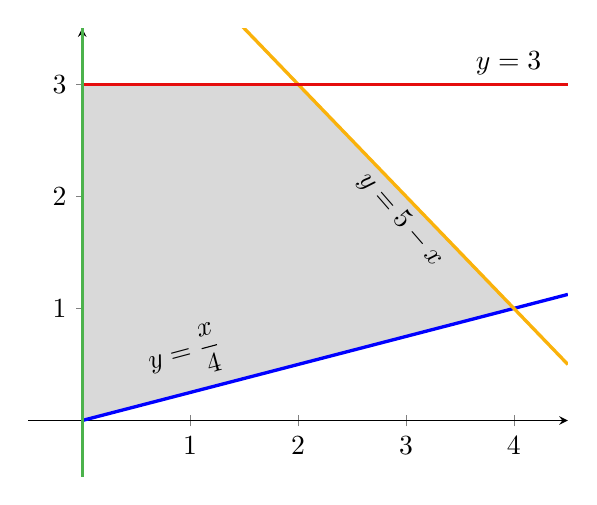
\begin{tikzpicture}
  \begin{axis}[
    axis lines=middle,
    xmin=-0.5,xmax=4.5,ymin=-0.5,ymax=3.5
  ]
  \addplot[very thick,blue, samples=300, domain=0:4.5, name path=A] {x/4}; 
  \addplot[very thick,yellow!70!red, samples=300, domain=0:4.5, name path=B] {5-x}; 
  \addplot[very thick,red!90!teal, samples=300, domain=0:4.5, name path=C] {3}; 
  \addplot[very thick,green!70!magenta, samples=300, domain=0:4.5, name path=D] coordinates{(0,-6) (0,6)};
  \addplot[gray!30] fill between[of=A and C,soft clip={domain=0:2}];
  \addplot[gray!30] fill between[of=A and B,soft clip={domain=2:4}];
\node [rotate=15] at (axis cs:  0.95,  .59) {$\displaystyle y=\frac{x}{4}$};
\node [rotate=-49] at (axis cs:  2.95,  1.79) {$y=5-x$};
\node [rotate=0] at (axis cs:  3.95,  3.19) {$y=3$};
  \end{axis}
\end{tikzpicture}

 \begin{parts}
\part[3] \label{part:one} One of the corner points of the feasible region is $(0,0)$. Find the other three corned points. Show Your work step by step and include explanations.
\fillwithdottedlines{5cm}
\bonuspart[1]  (Circle the one correct answer.) The feasible region shown above is:
\begin{oneparchoices}
	\choice bounded; 
	\choice unbounded.
	\end{oneparchoices}

\part[4] Find the maximum value of the objective function $10-4x+2y$ in the feasible region shown above. Please use the method described in class to solve this problem and show your work step by step.
\fillwithdottedlines{5cm}
\end{parts}	

%{\large{\bfseries{ Questions 3 and 4 are on the back.}}}
%\newpage







%%\setlength\fboxrule{2pt}\setlength\fboxsep{2mm}
%%\fbox{This part of the page is intentionally left blank.} You may use it as scrap paper for your calculations as you solve the problems in this quiz.

%%\fillwithdottedlines{12cm}



%%%%%%%%%%%%%%%%%%%%%%%%%%



\end{questions}

\end{document}                 